%==============================
\section{Related Work}\label{sec:related-work}




%==============================
\subsection{Multi-agent Task and Motion Planning}\label{subsec:multi-tamp}
Planning for multi-agent systems have two distinctive characteristics:
high-level task planning in the discrete task space,
and low-level motion planing in the continuous state space.
In particular,
given a team-wise task, task planning refers to the process of first decomposing this task into sub-tasks
and then assigning them to the team, see~\cite{torreno2017cooperative,gini2017multi, khamis2015multi} for comprehensive surveys.
Such tasks can have additional constraints,
such as time windows~\cite{luo2015distributed}, robot capacities~\cite{fukasawa2006robust},
and ordering constraints~\cite{boerkoel2013distributed, nunes2015multi}.
The optimization criteria can be single or multiple,
two of which are the most common:
MinSUM that minimizes the sum of robot costs over all robots~\cite{gini2017multi, luo2015distributed, fukasawa2006robust},
and MinMAX that minimizes the maximum cost of a robot over all robots~\cite{nunes2015multi},
similar to the \emph{makespan} of all tasks.
Typical solutions can be categorized into centralized methods such as
Mixed Integer Linear Programming (MILP)~\cite{torreno2017cooperative} and search-based methods~\cite{fukasawa2006robust}\todoliu{add an automatica \cite{FANG2022110228}};
and decentralized methods such as
market-based methods~\cite{luo2015distributed} and distributed constraint optimization (DCOP)~\cite{boerkoel2013distributed}.
However, since many task planning problems are in general NP-hard or even NP-complete~\cite{gini2017multi},
meta-heuristic approaches are used to gain computational efficiency,
e.g., local search~\cite{hoos2004stochastic} and genetic algorithms~\cite{khamis2015multi}.
One type of problem is particularly of relevance to this work,
namely the Multi-Vehicle Routing Problem (MVRP) in operation research~\cite{gini2017multi, khamis2015multi},
where a team of vehicles are deployed to provide services at a set of locations,
and the MinSum objective above is optimized.
Despite of the similarity,
this work considers a significantly more general specification of team-wise tasks,
which can include as special cases the vanilla formulation and its variants with
temporal and spatial constraints~\cite{boerkoel2013distributed, nunes2015multi}.
Moreover, collaborative tasks and synchronization during online execution are often neglected in the aforementioned work, where planning and execution are mostly decoupled.

On the other hand,
motion planning problem for multi-agent systems aims at designing cooperative control policies such that a team-wise control objective is reached,
e.g., collision-free navigation~\cite{lavalle2006planning}, formation~\cite{chen2005formation},
consensus~\cite{li2009consensus} and coverage~\cite{mesbahi2010graph}.
Such objectives are self-sustained but lacks a high-level purpose for task completion.
In this work, we extend these results by incorporating them into the team-wise task as collaborative sub-tasks.


%==============================
\subsection{Temporal Logic Tasks}\label{subsec:multi-ltl}

Temporal logic formulas can be used to specify complex robotic tasks,
such as Probabilistic Computation Tree Logic (PCTL) in~\cite{lahijanian2011temporal},
Linear Temporal Logics (LTL) in~\cite{kantaros2020stylus, schillinger2018simultaneous,
 guo2015multi, chen2011formal},
and counting LTL (cLTL) in~\cite{sahin2019multirobot}.
As summarized in Table~\ref{table:compare},
the most related work can be compared in the following four aspects:
(i) \emph{collaborative tasks}.
In a bottom-up fashion,~\cite{guo2015multi, tumova2016multi, guo2016task} assume local LTL tasks and dynamic environment,
where collaborative tasks are allowed in~\cite{guo2016task}.
In a top-down fashion,~\cite{kantaros2020stylus, schillinger2018simultaneous, luo2021temporal, sahin2019multirobot, jones2019scratchs} consider team-wise tasks,
but no direct collaboration among the agents;
(ii) the \emph{optimization criteria}.
Most aforementioned work~\cite{kantaros2020stylus, guo2016task, luo2021temporal, sahin2019multirobot, jones2019scratchs} optimizes
the summed cost of all agents,
while~\cite{schillinger2018simultaneous} evaluates a weighted balance between this cost and
the task completion time. 
Even though both objectives are valid,
we emphasize in this work the achievement of maximum efficiency by minimizing solely the completion time;
(iii) the \emph{synchronization requirement}.
Synchronization happens when two or more agents communicate regarding the starting time of next the next sub-task.
The work in~\cite{kantaros2020stylus, luo2021abstraction, sahin2019multirobot} requires
full synchronization before each sub-task due to the product-based solution,
while~\cite{schillinger2018simultaneous} imposes no synchronization by allowing
only independent sub-tasks and thus limiting efficiency.
This work however proposes an online synchronization strategy for sub-tasks
that satisfies both the strict partial ordering and the simultaneous collaboration.
As illustrated in Fig.~\ref{fig:concurrent},
this can improve greatly the concurrency and thus the efficiency of the multi-agent execution even further;
and lastly
(iv) the \emph{solution basis}.
Solutions based on solving a MILP as in~\cite{luo2021temporal, sahin2019multirobot, jones2019scratchs} often can not guarantee a feasible solution within a time budget,
while this work proposes an anytime algorithm that could return quickly a feasible
and near-optimal solution.
Last but not least,
instead of generating only a static team-wise plan as in the aforementioned work,
the proposed online adaptation algorithm can handle fluctuations in the task duration
and possible agent failures during execution.

%========================================
\begin{figure}[t!]
	\centering
	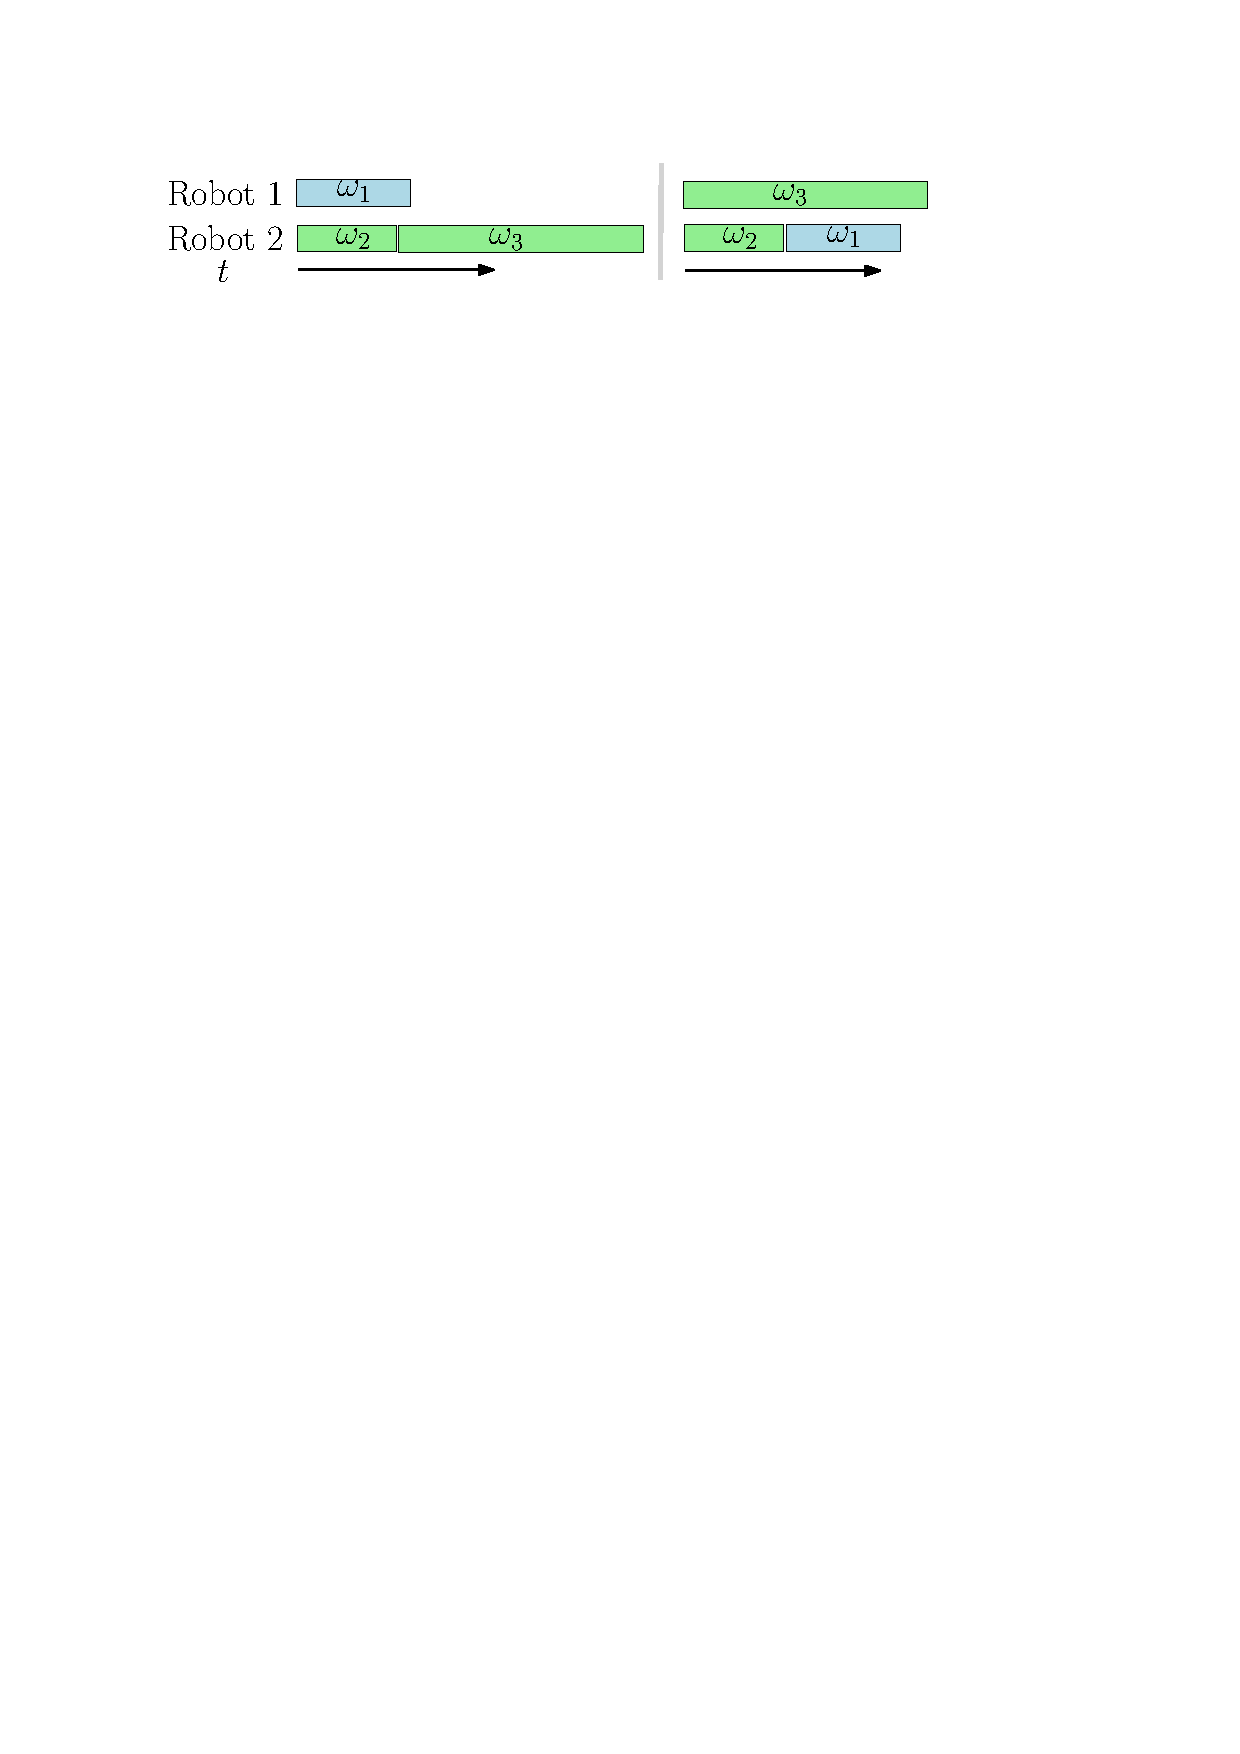
\includegraphics[width=0.95\linewidth]{figures/concurrent.pdf}
	%--------------------
	\caption{Comparison of the planning results based on decompositional states
		in~\cite{schillinger2018simultaneous} (\textbf{left}) and the partial ordering proposed in this work (\textbf{right}).
		Note that the sub-task~$\omega_3$ has to be {completed}
                after~$\omega_2$, while~$\omega_1$ is independent.}
		\label{fig:concurrent}
		%--------------------
\end{figure}
%========================================



%==============================
\subsection{Branch and Bound}\label{subsec:BnB-search}
\todoliu{remove here and add a short description in bnb search section:
Branch and bound (BnB) is a search paradigm to solve discrete and combinatorial optimization problems exactly~\cite{lawler1966branch, morrison2016branch}.
All candidate solutions are represented by a rooted tree within the solution space.
Via branching and bounding intelligently,
an efficient search strategy can be derived by pruning early branches that are provably
suboptimal. It has been successfully applied to various NP-hard problems, e.g.,
the traveling salesman problem~\cite{junger1995traveling},
multi-vehicle routing problem~\cite{gini2017multi, khamis2015multi},
and the job-shop scheduling problem~\cite{brucker1994branch}.
Different from the commonly-seen BnB algorithms that are applied to MILP directly,
we propose in this work a novel BnB search strategy \emph{specifically} designed
for the planning problem of multi-agent systems under complex temporal tasks.
It takes into account both the partial ordering constraints imposed by the temporal task,
and the synchronization constraints due to inter-agent collaboration.
}